\documentclass[10pt]{amsart}
%\usepackage{amsmath}
\usepackage[utf8]{inputenc}
\usepackage{graphicx}
\usepackage{xcolor}
\usepackage[legalpaper, margin=1.5in]{geometry}
\usepackage{fancyvrb}
\usepackage{url}
\usepackage{etoolbox}
\usepackage{hyperref}




% fonts
\input{ArtNouvc.fd}
\newcommand*\initfamily{\usefont{U}{ArtNouvc}{xl}{n}}
\usepackage[T1]{fontenc}
\usepackage{tgbonum} % change font


% from https://www.pinterest.co.uk/pin/88664686405122253/
\definecolor{C1}{RGB}{141, 125, 158} %purple
\definecolor{C2}{RGB}{163,156,147} % yellow
\definecolor{C3}{RGB}{99,151,153} % green
\definecolor{C4}{RGB}{195,106,99} % red
\definecolor{C5}{RGB}{124, 132, 128}
\definecolor{C6}{RGB}{67, 69, 75}

\hypersetup{
    colorlinks=false,
    linkcolor=C2,
    filecolor=magenta,      
    urlcolor=C3,
    pdftitle={Overleaf Example},
    pdfpagemode=FullScreen,
    }
    
    
\patchcmd{\section}{\normalfont}{\color{C5}}{}{}
\patchcmd{\subsection}{\normalfont}{\color{C5}}{}{}


\newcommand{\dfn}[1]{\bf  \color{C2}{#1}}


\renewcommand{\FancyVerbFormatLine}[1]{\color{C3}{>\,\,#1}}
    
\newtheorem{thm}{Theorem}

\newtheoremstyle{exercise}
{}                % Space above
{}                % Space below
{\color{C4}\slshape}        % Theorem body font % (default is "\upshape")
{}                % Indent amount
{\bfseries}       % Theorem head font % (default is \mdseries)
{:}               % Punctuation after theorem head % default: no punctuation
{ }               % Space after theorem head
{}                % Theorem head spec
\theoremstyle{exercise}
\newtheorem{exercise}{Exercise}


\newtheoremstyle{example}
{}                % Space above
{}                % Space below
{\color{C1}\slshape}        % Theorem body font % (default is "\upshape")
{}                % Indent amount
{\bfseries}       % Theorem head font % (default is \mdseries)
{.}               % Punctuation after theorem head % default: no punctuation
{ }               % Space after theorem head
{}                % Theorem head spec
\theoremstyle{example}
\newtheorem{example}{Example}

\newtheoremstyle{solution}
{}                % Space above
{}                % Space below
{\color{C5}}        % Theorem body font % (default is "\upshape")
{}                % Indent amount
{\bfseries }       % Theorem head font % (default is \mdseries)
{:}               % Punctuation after theorem head % default: no punctuation
{\newline}               % Space after theorem head
{}                % Theorem head spec
\theoremstyle{solution}
\newtheorem*{solution}{Solution}


\newcommand{\mcS}{\mathcal S}
\newcommand{\mcR}{\mathcal R}
\newcommand{\mcC}{\mathcal C}
\newcommand{\bS}{{\boldsymbol S}}
\newcommand{\bR}{{\boldsymbol R}}
\newcommand{\bC}{{\boldsymbol C}}
\newcommand{\ba}{{\boldsymbol a}}
\newcommand{\bb}{{\boldsymbol b}}
\newcommand{\bs}{{\boldsymbol s}}
\newcommand{\bff}{{\boldsymbol f}}
\newcommand{\br}{{\boldsymbol r}}
\newcommand{\bx}{{\boldsymbol x}}
\newcommand{\bt}{{\boldsymbol t}}
\newcommand{\bv}{{\boldsymbol v}}
\newcommand{\bu}{{\boldsymbol u}}
\newcommand{\bw}{{\boldsymbol w}}
\newcommand{\bc}{{\boldsymbol c}}
\newcommand{\be}{{\boldsymbol e}}
\newcommand{\bq}{{\boldsymbol q}}
\newcommand{\bphi}{{\boldsymbol \phi}}
\newcommand{\brho}{{\boldsymbol \rho}}
\newcommand{\btau}{{\boldsymbol \tau}}
\newcommand{\reals}{\mathbb R}
\newcommand{\ints}{\mathbb N}
\newcommand{\E}{\mathbb E}
\newcommand{\Prob}{\mathbb P}

\title{\Huge \color{C1} Basic statistical models}
\author{\color{C1} Ethan Levien}
\date{April 2022}

\begin{document}

\maketitle

\tableofcontents

%
% \section{Discrete Models}
% So far we have mostly encountered discrete distributions; that is, distributions for which we can enumerate the outcomes as $1,2,3,\dots$. Let's look at a few more discrete distributions that will be of use later on. 
% 
%  \subsection{Geometric distribution}
%  The {\dfn geometric distribution} emerges when we are interested in how long it takes to get a successes from a sequence of Bernoulli trials. 
%  
%  
    




%\begin{solution}
%The following code will estimate the mean and standard deviations for various values of $q$:
%\begin{Verbatim}
%def mean_std_bern(n,q):
%  sample = np.random.binomial(n,q,100)
%  return np.mean(sample),np.std(sample)
%
%# generates one hundred evenly spaced numbers between 0 and 1
%q_range = np.linspace(0,1,100)
%means = np.zeros(len(q_range))
%stds = np.zeros(len(q_range))
%for j in range(len(q_range)):
%  means[j],stds[j] = mean_std_bern(q_range[j])
%\end{Verbatim}
%Here is a plot of the mean compared to the prediction
%\begin{Verbatim}
%fig,ax = plt.subplots(figsize=(5,2))
%ax.plot(q_range,means)
%ax.plot(q_range,q_range,"k--")
%\end{Verbatim}
%and the standard deviations
%\begin{Verbatim}
%fig,ax = plt.subplots(figsize=(5,2))
%ax.plot(q_range,stds)
%ax.plot(q_range,np.sqrt((1-q_range)*q_range),"k--")
%\end{Verbatim}
%\end{solution}


  \section{Binomial Distribution}
A situation that often arrises is that we take many, say $N$, independent samples from a Bernoulli distribution. Now let $Y$ be the number of $1$s. Symbolically, 
\begin{equation}
Y = \sum_{i=1}^N y_i ,\quad y_i \sim {\rm Bernoulli}(q).
\end{equation}
 Then $Y$ follows {\dfn binomial distribution}:
\begin{equation}
Y \sim {\rm Binomial}(N,q)
\end{equation}
The binomial distribution has two parameters, $N$ and $p$. Now let's think about the probability distribution. The chance to find any particular configuration of $k$ ones is $q^k(1-q)^{N-k}$ because they are independent. For example
\begin{align}
P(y_1 = 1,y_2 = 0,y_3 = 1) &= P(y_1 = 1)P(y_2=0)P(y_3 =1) \\
&= q(1-q)q = q^2(1-q).
\end{align}
However, there are many configurations with $k$ ones, in-fact there are 
\begin{equation}
{N \choose k} = \frac{N!}{k!(N-k)!},
\end{equation}
and therefore 
\begin{equation}
P(Y=k) = {N \choose k}q^{k}(1-q)^{N-k}. 
\end{equation}
The binomial distribution has a mean and variance
\begin{equation}
\E[Y] = qN \quad\quad{\rm var}(Y) = Nq(1-q). 
\end{equation}
Binomial samples can be generated in numpy with
 \begin{Verbatim}
y = np.random.binomial(n,p,n_samples)
 \end{Verbatim}
 
 An important feature of the Bernoulli random variables is that the mean grows much faster in $N$ than the standard deviation. This means that when $N$ is very large, the deviations from the average will become very small relative to the mean. An important measure of variation relative to the mean is the coefficient of variation 
\begin{equation}
{\rm CV} = \frac{\sqrt{{\rm var}(Y)}}{\E[Y]}. 
\end{equation}
 
 
  \begin{example}
\href{https://colab.research.google.com/drive/1PPFwE4GUzsr707s3mPhGRs7-TYlHxND2#scrollTo=oaFLfi0JI4in&line=1&uniqifier=1}{Coefficient of variation}
\end{example}


 \begin{exercise}
\href{https://colab.research.google.com/drive/1PPFwE4GUzsr707s3mPhGRs7-TYlHxND2#scrollTo=vAmv5zV7gfE0}{Generating binomial samples}
\end{exercise}

\begin{exercise}
\href{https://colab.research.google.com/drive/1PPFwE4GUzsr707s3mPhGRs7-TYlHxND2#scrollTo=8cRVZNYtLOum}{Binomial election modeling}
\end{exercise}

You should recognize that the assumption of independence is very important here. The following example illustrates an instance where this may break down for an election model. It is a bit contrived, but this contrived example, which we sometimes refer to as {\dfn toy models}, can be very helpful when it comes to building our intuition. 
\begin{exercise}
\href{https://colab.research.google.com/drive/1PPFwE4GUzsr707s3mPhGRs7-TYlHxND2#scrollTo=cwE2yj2nqdYF&line=1&uniqifier=1}{More election modeling}
\end{exercise}

 

 
 
 \section{Uniform distribution and probability density}
 A uniform random variable, denoted  
 \begin{equation}
 Y \sim {\rm Uniform}(a,b)
 \end{equation}
 has an equal chance of taking any number in the interval $[a,b]$ (we assume $a<b$). Let $L=b-a$. This is distinct from other distributions we have encountered in that it is a {\dfn continuous distribution}, rather than discrete. For the uniform distribution, 
 \begin{equation}
 P(y_1\le Y \le y_2) = \frac{y_2-y_1}{L}
 \end{equation}
 for $a<y_1<y_2<b$. 
 That is, the chance for $Y$ to fall in any interval is simply the length of that interval. This insures that that the probability of $Y$ being somewhere in $[a,b]$ is one: $P(a\le Y\le b) = 1$. Note that as $y_2 \to y_1$, $P(y_1\le Y \le y_2) \to 0$. This tells us that the chance for $Y$ to take any specific value is $0$. Indeed, there are simply two many number (uncountably many) in any interval to assign positive probability to each. For continuous variables, it is sometimes useful to work with the density, $f(y)$ (we will use lower case letters for density and uppercase for probability distributions). $f(y)$ is the the probability per unit $Y$, meaning that if we look in a small interval 
 \begin{equation}
f(y)dy = P(y \le Y \le y+dy) = \frac{dy}{L}.
 \end{equation}
 Thus, for uniform distribution the density is $1/L$ if $y \in [a,b]$ and $0$ otherwise. 
 
 \subsection{Joint density and conditional density}
 
 Conditioning works for probability density just as it does for probability distributions. As an example, consider
 \begin{equation}
 Y \sim {\rm Uniform}(0,1)
 \end{equation}
 
 \begin{example}
\href{}{Conditioning with continuous variables} 
 \end{example}
 
 \subsection{Cumulative density function}
Sometimes it is useful to characterize a continuous distribution not by the density, but by the {\dfn cumulative distribution function (CDF)}, defined as 
\begin{equation}
F(y) = P(Y<y).
\end{equation}
What is the CDF of the uniform distribution? The {\dfn median} is the value $y_m$ for which $F(y_m) = 1/2$. What is the median of a Uniform distribution?  
  
  
  To better understand density and CDF, imagine a student says they will arrive at my office between noon and 3. Let $Y$ represent the time a student arrives, which we will model as a Uniform random variable. Then the density is $f(y) = 1/3$ which has units 1/hours. We can think of $f$ as the rate at which the CDF increases -- that is, it is the velocity of probability. 
  
  
  
  
  \section{Normal distribution and the central limit theorem}

In the previous example, we say that if we take the average of many Bernoulli random variables, we get a histogram that looks a lot like a ``bell curve" with a standard deviation was proportional to $1/\sqrt{n}$.

It turns out this is true when we add up \emph{any} sequence of independent and independent distributed  random variables which are not too pathological (actually it is also true for many sequences of random variables which are not independent). Since the ``bell curve" arrises in the limit where we sum or average many random variables,
\begin{equation}
Y = \frac{1}{N}\sum_{i=1}^Ny_i,
\end{equation}
it makes sense to approximate it with a continuous variable. We call this a Normal random variable
\begin{equation}
Y \sim {\rm Normal}(\mu,\sigma)
\end{equation}
can take on any number, positive or negative, decimal or integer. 
We can generate Normal random variables in python with
\begin{Verbatim}
np.random.normal(0,1)
\end{Verbatim}


We want to describe this random variable in terms of a probability distribution, but just as for the uniform distribution, the probability for $Y$ to equal any given value of $Y$ is zero.  For example, the chance that someone is six feet tall plus $h$ inches is going to decrease as $h$ gets very small, and the chance that someone is \emph{exactly} $6$ feet tall is zero (although it won't appear that way in data to to imprecision in our measurements). Therefore, instead of defining our model in terms of the chance that someone is exactly $Y$ feet tall, we define it in terms of a density. 
%This means if we want to know what an arbitrary probability is, we can sum over $f$:
%\begin{equation}
%P(y \le Y \le y+h) \approx  \sum_j f(y+hj/L)h/L
%\end{equation}
%(If know calculate, you will recognize this becomes an integral)
For the Normal distribution, the density is 
\begin{equation}
f(y) = \frac{1}{\sqrt{2\pi \sigma}}e^{-\frac{-(y-\mu)^2}{2\sigma}}.
\end{equation}
This is the classic bell curve shown in Figure \ref{fig:bellcurve}. 
Again, we can think of $f$ as the probability \emph{per unit of the random variable}, e.g. probability/feet.  

\begin{figure}[h]
\centering
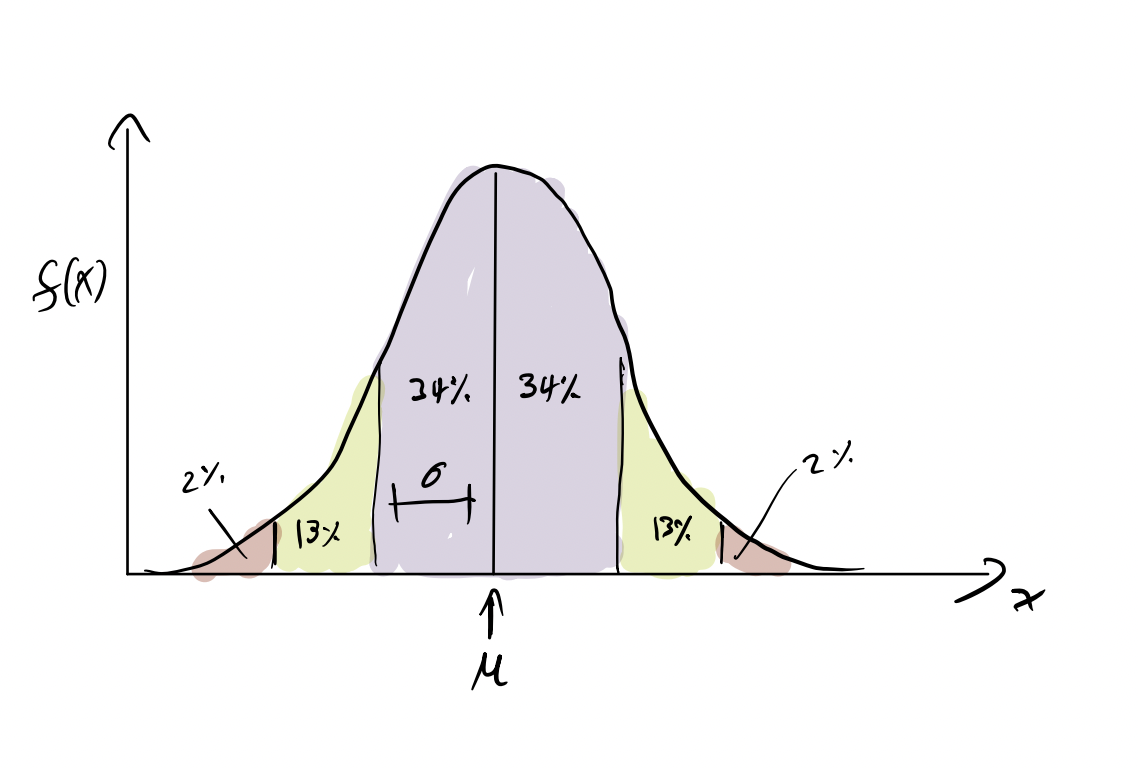
\includegraphics[width=0.8\textwidth]{bellcurve}
\caption{Probabilities in the Normal distribution}\label{fig:bellcurve}
\end{figure}

\begin{exercise}
\href{https://colab.research.google.com/drive/1PPFwE4GUzsr707s3mPhGRs7-TYlHxND2#scrollTo=qDKKEAeJXm87&line=1&uniqifier=1}{Comparing histograms}
\end{exercise}






\begin{example}
\href{https://colab.research.google.com/drive/1PPFwE4GUzsr707s3mPhGRs7-TYlHxND2#scrollTo=V7XdPehJX2Q3&line=1&uniqifier=1}{Working with Normal random variables}
\end{example}


\begin{exercise}
\href{https://colab.research.google.com/drive/1PPFwE4GUzsr707s3mPhGRs7-TYlHxND2#scrollTo=wq-MSEh7YARC&line=1&uniqifier=1}{Hemoglobin levels}
\end{exercise}

\subsection{Properties of Normal random variables}
Going forward, you will need to know the following properties of Normally distributed random variables. Let
\begin{equation}
Y_1 \sim {\rm Normal}(0,1),\quad Y_2 \sim {\rm Normal}(0,1)
\end{equation}
 Then
\begin{align}
aY_1 + b &\sim {\rm Normal}(b,|a|)\\
aY_1 + bY_2 &\sim {\rm Normal}(0,\sqrt{a^2 + b^2})
\end{align}
We can derive more general relationships from these identities:
\begin{equation}
Y \sim {\rm Normal}(\mu,\sigma)
\end{equation}
then 
\begin{equation}
aY + b \sim {\rm Normal}(a\mu+b,|a|\sigma).
\end{equation}
For example, if I say 
\begin{equation}
Y \sim {\rm Normal}(1,3)
\end{equation}
you should recognize that 
\begin{equation}
-4Y + 1 \sim {\rm Normal}(-3,4\times 3).
\end{equation}
%\begin{example}
%Show that if
%\begin{equation}
%Y_1 \sim {\rm Normal}(\mu_1,\sigma_1),\quad Y_2 \sim {\rm Normal}(\mu_2,\sigma_2)
%\end{equation}
%then
%\begin{equation}
%aY_1 + bY_2 + c \sim {\rm Normal}(\mu_1+\mu_2 + c,\sqrt{(a\sigma_1)^2 + (b\sigma_2)^2})
%\end{equation}
%\end{example}

\subsection{The central limit theorem}
We now return to the connection to sums of random variables and the Binomial distribution. The {\dfn central limit theorem} tells us that for a set of random variables $y_1,\dots,y_N$ with each have $\E[y_i] = \mu_y$ and ${\rm var}(y_i) = \sigma_y^2$,
\begin{equation}
Y = \sum_i^N y_i
\end{equation}
is approximately Normal with mean $\mu$ and variance $\sigma/\sqrt{n}$.
In other words Normal random variables emerge when we add up many small sources of randomness.

\section{Additional exercises}

The following exercise will help you practice the process of learning about a distribution by playing with simulations. 
 
 \begin{exercise} 
 \href{https://colab.research.google.com/drive/1PPFwE4GUzsr707s3mPhGRs7-TYlHxND2#scrollTo=YzDOf8zsU5x0&line=1&uniqifier=1}{Learning about a new distribution using simulations}
\end{exercise}

Just as it is important to understand where the Normal distributions comes from (this is what the central limit theorem tells us), it is important to understand what processes give rise to distributions which are not Normal. 
 \begin{exercise} 
 \href{https://colab.research.google.com/drive/1PPFwE4GUzsr707s3mPhGRs7-TYlHxND2#scrollTo=YzDOf8zsU5x0&line=1&uniqifier=1}{Model of income}
\end{exercise}
\end{document}

